\documentclass[11pt,letterpaper]{article}
\usepackage[T1]{fontenc}
\usepackage{lmodern}
\usepackage[margin=1in,headheight=15pt]{geometry}
\usepackage{amsmath,amssymb,amsthm,mathtools}
\usepackage{microtype,booktabs,graphicx,enumitem,fancyhdr,xcolor}
\usepackage{xurl}
\usepackage[colorlinks=true,linkcolor=blue!45!black,citecolor=blue!45!black,urlcolor=blue!45!black]{hyperref}
\newtheorem{theorem}{Theorem}[section]
\newtheorem{proposition}[theorem]{Proposition}
\newtheorem{lemma}[theorem]{Lemma}
\newtheorem{corollary}[theorem]{Corollary}
\theoremstyle{remark}
\newtheorem{remark}[theorem]{Remark}
\newcommand{\F}{\mathbf F}
\newcommand{\E}{\mathbf E}
\newcommand{\Prob}{\mathbf P}
\newcommand{\TV}{d_{\mathrm{TV}}}
\newcommand{\Law}{\mathcal L}
\newcommand{\Alt}{\operatorname{Alt}}
\newcommand{\Mat}{\operatorname{Mat}}
\newcommand{\GL}{\operatorname{GL}}
\newcommand{\Sp}{\operatorname{Sp}}
\newcommand{\rank}{\operatorname{rank}}
\newcommand{\nul}{\operatorname{null}}
\newcommand{\qb}[2]{\genfrac{[}{]}{0pt}{}{#1}{#2}_{q}}
\newcommand{\norm}[1]{\left\lVert #1\right\rVert}
\newcommand{\abs}[1]{\left|#1\right|}
\newcommand{\dd}{\mathrm d}
\newcommand{\pin}{497c1844e71393df41914f5b783d5dc9a618eb61}
\newcommand{\sourceurl}{https://github.com/VladimirReshetnikov/ProveIt/blob/497c1844e71393df41914f5b783d5dc9a618eb61/Analysis/GeneralizedRiemannHypothesis/Article/sections/spn.tex}
\setlist{itemsep=3pt,topsep=5pt}
\pagestyle{fancy}
\fancyhf{}
\fancyhead[L]{\small Rectangular symplectic blocks}
\fancyhead[R]{\small Uniform rank blindness}
\fancyfoot[C]{\thepage}
\setlength{\parskip}{3pt}
\setlength{\emergencystretch}{2em}
\hypersetup{pdftitle={Uniform rank blindness in rectangular symplectic blocks},pdfauthor={Research note prepared for Vladimir Reshetnikov}}

\title{\textbf{Uniform rank blindness\\in rectangular symplectic blocks}\\[6pt]
\large A sharp extension of the ProveIt GRH research article}
\author{Research note prepared for Vladimir Reshetnikov}
\date{27 November 2026}

\begin{document}
\maketitle
\begin{abstract}
We resolve the fixed rectangular gap left open in the symplectic part of the
ProveIt article and obtain estimates uniform over every aspect ratio.
Let $a\ge b\ge2$ be even, and project a uniformly random symplectic $b$-frame
in a nondegenerate $(a+b)$-space onto a fixed nondegenerate $a$-summand.
If $A$ is the resulting $a\times b$ matrix and $U$ has independent uniform
entries in $\F_q$, then
\[
 \TV(\rank A,\rank U)
 =\frac{\gamma_\infty}{(q-1)\gamma_{a-b}}q^{-a}
   +O_q(q^{-a-b}),\qquad
 \gamma_r=\prod_{i=1}^r(1-q^{-i}).
\]
In contrast, the full matrix distance tends, whenever $\min(a,b)\to\infty$,
to the positive constant
$\Delta_q=\theta_\infty(1-\eta_\infty)$, independently of the aspect ratio.
We compute its first correction and prove an accompanying signed-law
expansion for the quadratic residual $J_b-U^{\mathsf T}J_aU$.
All error constants depend only on $q$, even when $a-b$ grows arbitrarily.
The proof combines exact isometric-embedding counts, Gaussian binomial
moments, and quantitative inversion. The existing exact residual determinant
test is reproved and remains optimal at every finite size.
This is an unconditional finite-field theorem: its connection to the GRH
project is through the spanning and frame-statistics method, not an additional
zero hypothesis. Exact rational checks and independent exhaustive finite-field
enumeration accompany the proof. The new theorem is not Lean-formalized.
\end{abstract}

\section{The source question and the contribution}

The source for this continuation is the ProveIt repository at revision
\texttt{497c1844e713}, dated 27 November 2026 \cite{ProveIt}.
Its article consolidates 142 reports and records 997 labeled mathematical
results. The article distinguishes unconditional transfers, consequences
using Dirichlet GRH, and reductions with unproved target estimates.
The present note follows its unconditional symplectic thread, which abstracts
the spanning and frame-statistics ingredients of the source proof.

The precise outstanding case appears in the source label
\texttt{spn:q:symplectic}: for complementary nondegenerate frames with
$a-b$ fixed and positive, only a lower bound for the full matrix discrepancy
was available. The square case and a limit with $a-b\to\infty$ had been treated.
We supply one uniform theorem covering all of these shapes, including gaps
that vary without any bound as the smaller dimension increases.

\begin{center}
\small
\begin{tabular}{p{.37\textwidth}p{.55\textwidth}}
\toprule
Inspected source result & Contribution of this note \\
\midrule
Exact complementary-frame likelihood and optimal residual test
\newline\texttt{spn:thm:balanced}
& Reproved as the finite foundation; no novelty is claimed for this test.\\[4pt]
Square first corrections
\newline\texttt{spn:thm:square-block}
& A signed first correction with a uniform error for every rectangular gap.\\[4pt]
Increasingly tall rank bound $O_q(q^{b-a})$
\newline\texttt{spn:thm:nondeg-blind}
& The sharp leading term of order $q^{-a}$, with error $O_q(q^{-a-b})$.\\[4pt]
Square quadratic-defect law
\newline\texttt{spn:thm:defect-universality}
& Rectangular defect universality, with the same uniform error $O_q(q^{-a-b})$.\\
\bottomrule
\end{tabular}
\end{center}

Classical uniform rectangular rank laws and their convergence are treated by
Fulman and Goldstein \cite{FulmanGoldstein}. Exact counts of nonsingular
subspaces and disjoint pairs have antecedents in De Boeck and Van de Voorde
\cite{DeBoeck}. Those counts and the limiting iid laws are not claimed as new.
The contribution here is the uniform signed comparison of the symplectic
projection with an iid matrix of the \emph{same} size, and its consequences.
It is new relative to the inspected source; a targeted literature comparison
does not establish worldwide priority.

\section{Model and main results}

Fix a prime power $q$. For every positive even integer $r$, let $J_r$ be the
block diagonal alternating matrix with $r/2$ blocks
$\left(\begin{smallmatrix}0&1\\-1&0\end{smallmatrix}\right)$.
Thus the subscript of $J_r$ is its dimension. This convention also applies in
characteristic two, where an alternating matrix must have zero diagonal.

Let $a\ge b\ge2$ be even, put $d=a-b$, and consider
\[
 V=(\F_q^a,J_a)\perp(\F_q^b,J_b).
\]
Choose $g$ uniformly in $\Sp(V)$, apply it to the ordered standard basis of
the second summand, and write the resulting frame as
\begin{equation}\label{eq:gram}
 X=\begin{pmatrix}A\\B\end{pmatrix},\qquad
 A^{\mathsf T}J_aA+B^{\mathsf T}J_bB=J_b.
\end{equation}
Here $A\in\Mat_{a,b}(\F_q)$ and $B\in\Mat_b(\F_q)$.
Let $U$ be uniform on $\Mat_{a,b}(\F_q)$ and let $T_b$ be uniform on
$\Alt_b(\F_q)$. Define the quadratic residual and the four nullities
\begin{gather*}
 \Lambda(M)=J_b-M^{\mathsf T}J_aM,\\
 K_A=\dim\ker A,\quad K_U=\dim\ker U,\quad
 R_U=\dim\ker\Lambda(U),\quad R_T=\dim\ker T_b.
\end{gather*}
Both $R_U$ and $R_T$ are even. Since rank equals $b$ minus nullity, rank and
nullity have the same total variation discrepancy.
For laws on a countable set, our convention is
\[
 \TV(P,Q)=\frac12\sum_x|P(x)-Q(x)|=\sup_E|P(E)-Q(E)|.
\]

Use the products
\begin{equation}\label{eq:products}
 \gamma_r=\prod_{i=1}^r(1-q^{-i}),\quad
 \eta_r=\prod_{i=1}^r(1-q^{-2i}),\quad
 \theta_r=\prod_{i=1}^r(1-q^{-(2i-1)}).
\end{equation}
Empty products are one. Their infinite limits are positive, and
$\gamma_\infty=\eta_\infty\theta_\infty$.
Set
\begin{align}
 \alpha_{a,b}&=\frac{\eta_{a/2}\eta_{b/2}}{\eta_{(a+b)/2}},\label{eq:alpha}\\
 \Delta_q&=\theta_\infty(1-\eta_\infty)>0,\label{eq:delta}\\
 c_q&=\frac{\theta_\infty}{q^2-1}
       \bigl(q-(q+1)\eta_\infty\bigr)<0.\label{eq:cq}
\end{align}
The limiting iid rectangular and alternating nullity laws are
\begin{align}
 \pi_d(k)&=\frac{\gamma_\infty q^{-k(k+d)}}{\gamma_k\gamma_{k+d}}
       &&(k\ge0),\label{eq:pi}\\
 \lambda_q(2k)&=\frac{\theta_\infty q^{-k(2k-1)}}{\gamma_{2k}},
 &\lambda_q(2k+1)&=0.\label{eq:lambda}
\end{align}
Define signed summable sequences
\begin{align}
 \chi_d(k)&=\frac{q^d+1-q^{d+k}}{q-1}\,\pi_d(k),\label{eq:chi}\\
 \zeta_q(k)&=\frac{q+1-q^k}{q^2-1}\,\lambda_q(k).
 \label{eq:zeta}
\end{align}
Both have total mass zero.

\begin{theorem}[Uniform rank law]\label{thm:rank}
There is a finite constant depending only on $q$ such that, for every pair
of positive even integers $a\ge b$,
\begin{equation}\label{eq:rank-l1}
 \sum_{k\ge0}\left|
 \Prob(K_A=k)-\Prob(K_U=k)-q^{-a}\chi_{a-b}(k)
 \right|=O_q(q^{-a-b}).
\end{equation}
In particular,
\begin{equation}\label{eq:rank-tv}
 \boxed{\displaystyle
 \TV(\rank A,\rank U)
 =\frac{\gamma_\infty}{(q-1)\gamma_{a-b}}q^{-a}
       +O_q(q^{-a-b}).}
\end{equation}
The constants are independent of $a$, $b$, and $a-b$.
As $b\to\infty$, testing for full column rank is asymptotically optimal
among all tests that use only rank.
\end{theorem}

\begin{theorem}[Uniform quadratic-defect law]\label{thm:defect}
For the same parameter range,
\begin{equation}\label{eq:defect-l1}
 \sum_{k\ge0}\left|
 \Prob(R_U=k)-\Prob(R_T=k)-q^{-a}\zeta_q(k)
 \right|=O_q(q^{-a-b}),
\end{equation}
and consequently
\begin{equation}\label{eq:defect-tv}
 \TV(R_U,R_T)=\frac{q\theta_\infty}{q^2-1}q^{-a}
               +O_q(q^{-a-b}).
\end{equation}
\end{theorem}

\begin{theorem}[Persistent dependence at every aspect ratio]\label{thm:full}
The event $\det\Lambda(M)=0$ is an exactly optimal event for distinguishing
$A$ from $U$, at every finite $a,b$. More precisely,
\begin{align}
 \TV(A,U)
  &=(1-\alpha_{a,b})\Prob(\Lambda(U)\text{ nonsingular})\label{eq:full-exact}\\
  &=(1-\alpha_{a,b})\left(
    \theta_{b/2}+\frac{q\theta_\infty}{q^2-1}q^{-a}\right)
       +O_q(q^{-a-b}).\label{eq:full-centered}
\end{align}
In particular,
\begin{equation}\label{eq:full-expansion}
 \boxed{\displaystyle
 \TV(A,U)=\Delta_q+c_q(q^{-a}+q^{-b})
                  +O_q\bigl((q^{-a}+q^{-b})^2\bigr).}
\end{equation}
Thus $\TV(A,U)\to\Delta_q>0$ as $\min(a,b)\to\infty$, without an
assumption on the aspect ratio. The exact optimality assertion and
\eqref{eq:full-exact} are antecedents from the source; the uniform
expansions are the extension proved here.
\end{theorem}

\begin{remark}[Scope of the uniformity]
The field $\F_q$ is fixed. The theorem makes no assertion uniform as
$q\to\infty$. It permits $a-b$ to be zero, a fixed positive even integer,
or any function tending to infinity, however quickly. Interchanging the
source and target frames and transposing their pairing matrix gives the
rank and full-matrix conclusions when $a<b$, with $q^{-\max(a,b)}$ in the rank leading term
and $\gamma_{|a-b|}$ in its coefficient. Indeed, the transpose of
$Y^{\mathsf T}JgX$ is $-X^{\mathsf T}Jg^{-1}Y$, and $g^{-1}$ is again
uniform; fixed invertible coordinate changes preserve ranks and distances
from a uniform matrix. The defect theorem is stated with the smaller
frame as source. This does not cover frames with
growing radicals or a complement dimension independent of the source size.
\end{remark}

\section{Exact finite counts}

\subsection{Isometric embeddings}

The Gaussian binomial coefficient $\qb nj$ counts $j$-subspaces of $\F_q^n$;
it is zero for $j<0$ or $j>n$. Let $D$ be even. The number of isometric
injections of a prescribed alternating $j$-space of rank $2s$ into a
nondegenerate $D$-space is denoted by $E_D(j,s)$.
Put
\begin{equation}\label{eq:phi}
 \Phi_D(j,s)=
 \begin{cases}
 \displaystyle\prod_{i=D/2-j+s+1}^{D/2}(1-q^{-2i}),&j-s\le D/2,\\
 0,&j-s>D/2.
 \end{cases}
\end{equation}
We always restrict $s$ to $0\le2s\le j$.

\begin{lemma}[Embedding count]\label{lem:embedding}
For all the above parameters,
\begin{equation}\label{eq:embedding}
 E_D(j,s)=q^{Dj-\binom j2}\Phi_D(j,s).
\end{equation}
When embeddings exist, the symplectic group acts transitively on them.
\end{lemma}

\begin{proof}
Split the prescribed space into a nondegenerate $2s$-space and a radical of
dimension $r=j-2s$. An ordered symplectic basis of the nondegenerate part
embeds in $|\Sp_D(q)|/|\Sp_{D-2s}(q)|$ ways. In its orthogonal complement,
an independent isotropic ordered $r$-frame can be chosen successively in
\[
 \prod_{i=0}^{r-1}\bigl(q^{D-2s-i}-q^i\bigr)
\]
ways. It exists exactly when $r\le D/2-s$. Substituting
\[
 |\Sp_{2h}(q)|=q^{h^2}\prod_{i=1}^h(q^{2i}-1)
             =q^{h(2h+1)}\eta_h
\]
and collecting factors proves \eqref{eq:embedding}. A basis of any
embedded isotropic space can be completed to symplectic pairs by successively
choosing partners with prescribed pairings. Completing both embeddings to
symplectic bases gives an element carrying one to the other.
No division by two is used.
\end{proof}

The isometry group of the prescribed $j$-space of rank $2s$ has order
\begin{equation}\label{eq:aut}
 D(j,s)=|\Sp_{2s}(q)|\,|\GL_{j-2s}(q)|\,q^{2s(j-2s)}.
\end{equation}
Indeed, relative to a nondegenerate part followed by its radical, its
matrices have the form
$\left(\begin{smallmatrix}P&0\\R&S\end{smallmatrix}\right)$,
where $P$ is symplectic, $S$ is invertible, and $R$ is arbitrary.
Consequently the number of $j$-subspaces of a symplectic $b$-space of
restricted rank $2s$ is
\begin{equation}\label{eq:N}
 N_b(j,s)=\frac{E_b(j,s)}{D(j,s)}.
\end{equation}
If $H$ is uniform in $\Alt_j(\F_q)$, orbit counting also gives
\begin{equation}\label{eq:H}
 \Prob(\rank H=2s)=\frac{|\GL_j(q)|}{q^{\binom j2}D(j,s)}.
\end{equation}
As $|\GL_j(q)|=q^{j^2}\gamma_j$, comparison yields the useful identity
\begin{equation}\label{eq:N-averaging}
 N_b(j,s)=\frac{q^{j(b-j)}}{\gamma_j}
             \Prob(\rank H=2s)\Phi_b(j,s).
\end{equation}

\subsection{The residual likelihood and its sign}

\begin{proposition}[Exact source likelihood, reproved]\label{prop:likelihood}
If $\Lambda(M)$ has nullity $2\ell$, then
\begin{equation}\label{eq:likelihood}
 q^{ab}\Prob(A=M)=\alpha_{a,b}F_q(\ell),\qquad
 F_q(\ell)=\sum_{t=\ell}^{2\ell}
    \qb{2\ell}t\frac{q^{-t(t+1)/2}}{\eta_{t-\ell}}.
\end{equation}
The likelihood is less than one exactly when $\ell=0$, and greater than
one for every $\ell\ge1$.
\end{proposition}

\begin{proof}
The Gram equation \eqref{eq:gram} makes $X$ automatically injective: if
$Xv=0$, then $J_bv=X^{\mathsf T}J_{a+b}Xv=0$, so $v=0$.
By Lemma~\ref{lem:embedding}, $X$ is uniform among
$E_{a+b}(b,b/2)$ frames with this Gram matrix.
For a given $A=M$, a completion $B$ satisfies
$B^{\mathsf T}J_bB=\Lambda(M)$. Its kernel lies in the radical of
$\Lambda(M)$. If its dimension is $t$, its quotient has dimension $b-t$
and rank $b-2\ell$, and embeds into the $b$-space exactly when
$\ell\le t\le2\ell$. Thus the number of completions is
\[
 \sum_{t=\ell}^{2\ell}\qb{2\ell}t E_b(b-t,b/2-\ell).
\]
Formula \eqref{eq:embedding} turns its summand into
\[
 \qb{2\ell}t q^{b(b+1)/2-t(t+1)/2}
                    \frac{\eta_{b/2}}{\eta_{t-\ell}}.
\]
Division by the total frame count proves \eqref{eq:likelihood}.

The product constant satisfies $\eta_\infty\le\alpha_{a,b}<1$:
$\eta_{(a+b)/2}/\eta_{a/2}$ is a product of $b/2$ factors, each larger
than the corresponding factor in $\eta_{b/2}$. For $\ell=0$, $F_q(0)=1$.
For $\ell=1$,
\[
 F_q(1)=1+\frac q{q^2-1},\qquad
 \eta_\infty\ge 1-\sum_{i\ge1}q^{-2i}
                =\frac{q^2-2}{q^2-1}.
\]
The resulting lower bound minus one is
$(q^3-q^2-2q+1)/(q^2-1)^2>0$ for all $q\ge2$.
If $\ell\ge2$, the term $t=\ell$ alone gives
\[
 F_q(\ell)\ge q^{\ell^2-\ell(\ell+1)/2}
              =q^{\ell(\ell-1)/2}\ge q,
\]
so $\alpha_{a,b}F_q(\ell)\ge q\eta_\infty>1$.
\end{proof}

The excess mass is therefore exactly on the singular residuals. On the
complement the likelihood is the constant $\alpha_{a,b}$, which proves
\eqref{eq:full-exact} and the exact optimality assertion in
Theorem~\ref{thm:full}. The task remaining is to obtain uniform laws for
the two nullities; approximating the entire Gram matrix is unnecessary.

\section{Four exact kernel-moment formulas}

For an integer-valued random variable $K\ge0$, define its Gaussian binomial
moment of order $j$ by $\E\qb Kj$. This is the expected number of
$j$-subspaces in a kernel when $K$ is its dimension. Write
\[
 m_j^{(d)}=\frac{q^{-j(j+d)}}{\gamma_j},\qquad
 m'_j=\frac{q^{-j(j-1)/2}}{\gamma_j}.
\]
In expectations involving $\Phi_D$, let $H$ be uniform on
$\Alt_j(\F_q)$ and set $2s=\rank H$.

\begin{lemma}[Exact moment identities]\label{lem:moments}
For $0\le j\le b$,
\begin{align}
 \mu_j:=\E\qb{K_A}j
   &=m_j^{(d)}\E_H\frac{\Phi_b(j,s)^2}{\Phi_{a+b}(j,s)},
 &\mu_j^0:=\E\qb{K_U}j
   &=m_j^{(d)}\E_H\Phi_b(j,s),\label{eq:rank-moments}\\
 \nu_j:=\E\qb{R_U}j
   &=m'_j\E_H\bigl(\Phi_a(j,s)\Phi_b(j,s)\bigr),
 &\nu_j^0:=\E\qb{R_T}j
   &=m'_j\E_H\Phi_b(j,s).\label{eq:defect-moments}
\end{align}
The denominator in \eqref{eq:rank-moments} is always positive.
\end{lemma}

\begin{proof}
Fix a $j$-subspace $K$ of the source with restricted rank $2s$. Its image
under the random symplectic frame is uniform among the
$E_{a+b}(j,s)$ prescribed-Gram frames. Its $A$ component vanishes exactly
when this image lies in the second summand, which allows $E_b(j,s)$ choices.
Therefore
\[
 \mu_j=\sum_s N_b(j,s)\frac{E_b(j,s)}{E_{a+b}(j,s)},\qquad
 \mu_j^0=\qb bjq^{-aj}.
\]
Use \eqref{eq:N-averaging} and \eqref{eq:embedding} for the first two
identities. Since $j\le b\le(a+b)/2$, every type in the denominator is
feasible.

For the residual, the condition $K\subseteq\ker\Lambda(U)$ says
\[
 x^{\mathsf T}J_by=(Ux)^{\mathsf T}J_a(Uy)
                \quad(x\in K,\ y\in\F_q^b).
\]
It forces $U|_K$ to be injective: if $Ux=0$ with $x\in K$, the left side
vanishes for every $y$, whence $x=0$. There are $E_a(j,s)$ isometric
injections on $K$. After one has been fixed, every vector in a complementary
basis of the source has $j$ independent prescribed pairings, hence
$q^{a-j}$ possible images. This gives
\[
 \nu_j=\sum_s N_b(j,s)E_a(j,s)
                         q^{(a-j)(b-j)-ab}.
\]
For a uniform alternating matrix, killing $K$ imposes
$bj-j(j+1)/2$ independent linear conditions, so
\[
 \nu_j^0=\qb bj q^{-bj+j(j+1)/2}.
\]
Substitute \eqref{eq:N-averaging} once more.
\end{proof}

These are finite identities. They already determine all four distributions,
because the transform $p_k\mapsto\sum_{k\ge j}\qb kjp_k$ is triangular
with diagonal one. They supply the exact rational calculation in the archive.

\section{Uniform first-order moment expansions}

\subsection{A product estimate valid at infeasible types}

For $H\in\Alt_j(\F_q)$ of rank $2s$, put
\begin{equation}\label{eq:W}
 W(H)=\frac{q^{2(j-s)}-1}{q^2-1}.
\end{equation}
For any even $D$, on the feasible range the sum of the omitted factors in
\eqref{eq:phi} is exactly $q^{-D}W$. The elementary product inequalities
\[
 0\le\prod_i(1-x_i)-\left(1-\sum_i x_i\right)
     \le\frac12\left(\sum_i x_i\right)^2
       \quad(0\le x_i\le1)
\]
give
\begin{equation}\label{eq:phi-expand}
 \Phi_D=1-q^{-D}W+O_q(q^{-2D}q^{4j}),\qquad
 |1-\Phi_D|\le q^{-D}W.
\end{equation}
These estimates hold on the infeasible range too: there $\Phi_D=0$ and
$q^{-D}W\ge1$, so $|q^{-D}W-1|\le(q^{-D}W)^2$.
Also $0\le\Phi_D\le1$ and $W\le q^{2j}/(q^2-1)$.

Set
\[
 \tau=q^{-b},\qquad \rho=q^{-a},\qquad \sigma=\rho\tau=q^{-a-b}.
\]
For $j\le b$, $\Phi_{a+b}\ge\eta_\infty$, and
$|\Phi_{a+b}^{-1}-1|\le\eta_\infty^{-1}\sigma W$.
Using $\rho\le\tau$ in \eqref{eq:phi-expand} yields
\begin{align}
 \frac{\Phi_b^2}{\Phi_{a+b}}-\Phi_b
     &=-\tau W+O_q(\tau^2q^{4j}),\label{eq:prod-rank}\\
 \Phi_b(\Phi_a-1)
     &=-\rho W+O_q(\sigma q^{4j}).\label{eq:prod-defect}
\end{align}
For example, the second line follows by writing
$\Phi_a-1=-\rho W+O_q(\rho^2q^{4j})$ and bounding
$\rho W(1-\Phi_b)$ by $\rho\tau W^2$.
Both remainders vanish identically at $j=0$.

For $j\ge1$, a fixed nonzero vector is killed by a uniform alternating
$j$-matrix with probability $q^{-(j-1)}$. Thus
\[
 \E_Hq^{\dim\ker H}=1+(q^j-1)q^{1-j}.
\]
Since $2(j-s)=j+\dim\ker H$, this gives
\begin{equation}\label{eq:EW}
 \E_HW(H)=\frac{q^j-1}{q-1}.
\end{equation}
It holds also for $j=0$, with both sides zero.

\begin{lemma}[Uniform moment remainders]\label{lem:moment-errors}
For $0\le j\le b$,
\begin{align}
 \mu_j-\mu_j^0
   &=-\tau m_j^{(d)}\frac{q^j-1}{q-1}
       +O_q\left(\sigma q^{-j^2+4j}/\gamma_j\right),\label{eq:muerror}\\
 \nu_j-\nu_j^0
   &=-\rho m'_j\frac{q^j-1}{q-1}
       +O_q\left(\sigma m'_jq^{4j}\right).\label{eq:nuerror}
\end{align}
\end{lemma}

\begin{proof}
Apply \eqref{eq:prod-rank}--\eqref{eq:EW} to
Lemma~\ref{lem:moments}. For the rank error, the initially available
bound is $O_q(\tau^2m_j^{(d)}q^{4j})$. At $j=0$ it is zero.
At $j\ge1$,
\begin{equation}\label{eq:uniform-key}
 \tau^2q^{-j(j+d)}
       \le\tau^2q^{-d}q^{-j^2}
       =\sigma q^{-j^2}.
\end{equation}
This gains the factor needed to make the error uniform for arbitrarily
large $d$. The defect error is already of the desired size.
\end{proof}

\subsection{The signed correction laws}

For completeness, ordinary rank counting gives the finite iid probabilities
for an $(n+d)\times n$ matrix:
\begin{equation}\label{eq:finite-iid}
 p_{n,d}(k)=q^{-k(k+d)}
       \frac{\gamma_{n+d}\gamma_n}
            {\gamma_{n-k}\gamma_k\gamma_{k+d}},\quad 0\le k\le n.
\end{equation}
Choose the kernel, and then an injection from its quotient, to obtain this
formula. For a uniform alternating $2h\times2h$ matrix, choosing the radical
and a nonsingular form on its quotient gives
\begin{equation}\label{eq:finite-alt}
 t_{2h}(2k)=q^{-k(2k-1)}
        \frac{\gamma_{2h}}{\gamma_{2k}\eta_{h-k}},\quad 0\le k\le h.
\end{equation}
The other probabilities are zero.
These formulas converge to \eqref{eq:pi} and \eqref{eq:lambda}.
Their tails are bounded by constants depending only on $q$ times
$q^{-k(k+d)}$ and $q^{-k(2k-1)}$, respectively. Hence the limit laws have
total mass one, and their Gaussian moments can be obtained by dominated
convergence from the finite kernel counts:
\begin{equation}\label{eq:limit-moments}
 \sum_k\qb kj\pi_d(k)=m_j^{(d)},\qquad
 \sum_k\qb kj\lambda_q(k)=m'_j.
\end{equation}

Let $\xi_d=q^{-d}\chi_d$. The elementary identities
\begin{gather}
 (q^k-q^j)\qb kj=q^j(q^{j+1}-1)\qb k{j+1},\label{eq:tilt}\\
 (q^{j+1}-1)m_{j+1}^{(d)}=q^{-j-d}m_j^{(d)},\qquad
 (q^{j+1}-1)m'_{j+1}=qm'_j\nonumber
\end{gather}
show that
\begin{align}
 \sum_k\qb kj\xi_d(k)
     &=-m_j^{(d)}\frac{q^j-1}{q-1},\label{eq:xi-mom}\\
 \sum_k\qb kj\zeta_q(k)
     &=-m'_j\frac{q^j-1}{q-1}.\label{eq:zeta-mom}
\end{align}
At $j=0$ these say that both signed sequences have total mass zero.
Thus the proposed corrections have exactly the first-order moments in
Lemma~\ref{lem:moment-errors}. We next justify passage from moments to
the entire distributions, with a uniform error.

\section{Quantitative inversion}

\subsection{Direct inversion for the rank law}

The Gaussian binomial inversion formula is
\begin{equation}\label{eq:inversion}
 p_k=\sum_{j\ge k}(-1)^{j-k}q^{\binom{j-k}2}\qb j k\mu_j,
       \qquad \mu_j=\sum_{z\ge j}\qb zj p_z.
\end{equation}
For finite support this follows from
$\qb zj\qb jk=\qb zk\qb{z-k}{j-k}$ and the finite $q$-binomial theorem.
The absolute column sum of its inverse matrix is exactly
\begin{equation}\label{eq:invcol}
 \sum_{k=0}^j q^{\binom{j-k}2}\qb jk
   =\prod_{i=0}^{j-1}(1+q^i)
   \le C(q)q^{j(j-1)/2},
\end{equation}
where $C(q)=2\prod_{i\ge1}(1+q^{-i})<\infty$ also bounds the $j=0$ case.

Apply this to the signed measure
\[
 \mathcal R=\Law(K_A)-\Law(K_U)-\tau\xi_d
            =\Law(K_A)-\Law(K_U)-\rho\chi_d.
\]
Its moment $e_j$ satisfies $|e_j|\le C_q\sigma q^{-j^2+4j}$ for
$j\le b$, since $\gamma_j\ge\gamma_\infty$.
For $j>b$, the two finite distributions have moment zero, so
\[
 |e_j|=\tau m_j^{(d)}\frac{q^j-1}{q-1}
       \le C_q\sigma q^{-j^2+2j}.
\]
Indeed, after division by $\sigma q^{-j^2}$, the remaining power is
$q^{a-dj+j}=q^{b+d(1-j)+j}\le q^{2j}$ because $b<j$ and $d\ge0$.
Consequently \eqref{eq:invcol} gives
\begin{equation}\label{eq:rank-remainder}
 \norm{\mathcal R}_1
 \le C_q\sum_{j\ge0}q^{j(j-1)/2}|e_j|
 \le C'_q\sigma\sum_{j\ge0}q^{-j^2/2+7j/2}
 =O_q(\sigma).
\end{equation}

There is no hidden infinite inversion assumption here. For $k\ge1$,
$|\chi_d(k)|\le C_q q^{-k^2+k}$ uniformly in $d$, and $\chi_d(0)$ is
uniformly bounded. After exchanging the two sums in \eqref{eq:inversion},
the absolute inner sum is bounded using \eqref{eq:invcol} by a constant
times $q^{z(z-1)/2}$. Multiplication by $q^{-z^2+z}$ is summable.
This justifies inversion and all exchanges for the signed correction;
the other laws are finitely supported. Thus \eqref{eq:rank-remainder}
proves \eqref{eq:rank-l1}.

The only positive value of $\chi_d$ is at zero, where
\[
 \chi_d(0)=\frac{\gamma_\infty}{(q-1)\gamma_d}.
\]
For $k\ge1$, $q^d+1-q^{d+k}\le0$; equality occurs at $k=1$ only when
$q=2,d=0$. Since the signed mass totals zero,
$\tfrac12\norm{\chi_d}_1=\chi_d(0)$. The reverse triangle inequality
for the $\ell^1$ norm proves \eqref{eq:rank-tv}. The probability difference
of the event $K=0$ has this same leading term, proving its asymptotic
optimality. This completes the proof of Theorem~\ref{thm:rank}.

\subsection{Even-grid inversion for the defect}

Direct Gaussian inversion does not give a summable error for the slower
alternating tails. The even support supplies the stronger interpolation
estimate needed here. Put $b=2h$ and, for $0\le k\le h$, define
\[
 L_{k,h}(x)=\prod_{\substack{0\le r\le h\\r\ne k}}
                   \frac{x-q^{2r}}{q^{2k}-q^{2r}}.
\]
This polynomial takes value one at $q^{2k}$ and zero at all other points
of the finite even grid.

\begin{lemma}[Even-grid coefficient and tail bounds]\label{lem:interpolation}
For every $i\ge0$,
\begin{equation}\label{eq:coeff}
 |[x^i]L_{k,h}(x)|
    \le\eta_\infty^{-3}q^{-k(k+1)}q^{-i(i-1)}.
\end{equation}
For even $z>b$,
\begin{equation}\label{eq:Ltail}
 |L_{k,h}(q^z)|
    \le\eta_\infty^{-2}q^{hz-h(h+1)-k(k-1)}.
\end{equation}
\end{lemma}

\begin{proof}
After each factor is written as a constant times $1-xq^{-2r}$,
the absolute constant prefactor is
$q^{-k(k+1)}/(\eta_k\eta_{h-k})$.
The sum of all products of $i$ distinct members of
$1,q^{-2},q^{-4},\ldots$ is $q^{-i(i-1)}/\eta_i$.
To see this, remove the staircase $0,1,\ldots,i-1$ from the increasing
indices and sum the resulting nonnegative gaps. This proves
\eqref{eq:coeff}. For \eqref{eq:Ltail}, each of the $h$ numerator factors
is at most $q^z$, while the denominator has absolute value
$q^{h(h+1)+k(k-1)}\eta_k\eta_{h-k}$.
\end{proof}

Let
\[
 \mathcal D=\Law(R_U)-\Law(R_T)-\rho\zeta_q.
\]
By \eqref{eq:nuerror} and \eqref{eq:zeta-mom}, its Gaussian moment
remainder is at most $C_q\sigma m'_jq^{4j}$ for $j\le b$.
Counting maps $\F_q^i\to\F_q^z$ by their image gives
\begin{equation}\label{eq:power}
 q^{iz}=\sum_{j=0}^i\left(\prod_{r=0}^{j-1}(q^i-q^r)\right)\qb zj.
\end{equation}
For $i\le h$, the absolute power moment of $\mathcal D$ is therefore
bounded by
\begin{equation}\label{eq:powererror}
 C_q\sigma\sum_{j=0}^i q^{-j(j-1)/2+(i+4)j}
       \le C'_q\sigma q^{i(i+9)/2}.
\end{equation}
The terms measured backwards from $j=i$ decrease at least geometrically,
so the last constant is independent of $i$.
Combining \eqref{eq:coeff} and \eqref{eq:powererror} yields
\begin{equation}\label{eq:inside}
 \left|\sum_zL_{k,h}(q^z)\mathcal D(z)\right|
 \le C_q\sigma q^{-k(k+1)}
       \sum_{i\ge0}q^{-i^2/2+11i/2}
 \le C'_q\sigma q^{-k(k+1)}.
\end{equation}

The finite distributions are supported on the interpolation grid, but the
signed correction has an infinite tail, which must be included. From
\eqref{eq:lambda}--\eqref{eq:zeta}, for even $z$,
$|\zeta_q(z)|\le C_q q^{-z(z-3)/2}$. Hence
\eqref{eq:Ltail} gives
\begin{align*}
 \rho\sum_{k=0}^h\sum_{\substack{z>b\\z\ \mathrm{even}}}
       |L_{k,h}(q^z)\zeta_q(z)|
 &\le C_q\rho q^{-h^2+1}
 \le C'_q\rho q^{-b}=O_q(\sigma).
\end{align*}
For the first inequality, at $z=2h+2$ the exponent not involving $k$ is
$-h^2+1$, and later terms have a uniform geometric decay; also
$\sum_kq^{-k(k-1)}<\infty$.
For the second, $2h-h^2+1\le2$ for every integer $h\ge1$.
The direct tail $\rho\sum_{z>b}|\zeta_q(z)|$ is smaller still.
Summing \eqref{eq:inside} over $k$, then adding both tails, proves
\eqref{eq:defect-l1}.

The only positive mass of $\zeta_q$ is at zero, with value
$q\theta_\infty/(q^2-1)$, because every positive possible nullity is
at least two. Its total mass is zero, so the reverse triangle inequality
gives \eqref{eq:defect-tv}. This proves Theorem~\ref{thm:defect}.

\section{The full distance and its meaning}

The finite alternating probability of nonsingularity is
$\Prob(R_T=0)=\theta_{b/2}$ by \eqref{eq:finite-alt}.
Theorem~\ref{thm:defect}, evaluated at zero, gives
\[
 \Prob(\Lambda(U)\text{ nonsingular})
    =\theta_{b/2}+\rho\frac{q\theta_\infty}{q^2-1}
       +O_q(\sigma).
\]
Insert this in the exact identity \eqref{eq:full-exact}; since
$0<1-\alpha_{a,b}<1$, the error remains $O_q(\sigma)$.
This proves \eqref{eq:full-centered}.

The product tails in \eqref{eq:products} give, uniformly as the dimensions
vary,
\begin{align*}
 \alpha_{a,b}
   &=\eta_\infty\left(1+\frac{\rho+\tau}{q^2-1}
                 +O_q((\rho+\tau)^2)\right),\\
 \theta_{b/2}
   &=\theta_\infty\left(1+\frac{q\tau}{q^2-1}
                    +O_q(\tau^2)\right).
\end{align*}
For example, the omitted even tail has sum $q^{-b}/(q^2-1)$ and
quadratic error $O_q(q^{-2b})$; the odd tail has sum
$q^{1-b}/(q^2-1)$. The denominator product in $\alpha_{a,b}$ contributes
only $O_q(\rho\tau)$ to this first-order expansion.
Multiplication proves \eqref{eq:full-expansion} with the constant
\eqref{eq:cq}.

To check its sign, $\eta_\infty>q/(q+1)$.
For $q>2$, the lower bound $(q^2-2)/(q^2-1)$ is already larger than
$q/(q+1)$. At $q=2$ the product inequality is strict, since at least
two omitted quantities are positive, so $\eta_\infty>2/3$.
Thus $c_q<0$, completing Theorem~\ref{thm:full}.

\begin{corollary}[A statistical separation]\label{cor:testing}
With equal prior probabilities for the two models, the best success
probability using the entire matrix is
\[
 \frac12+\frac12\TV(A,U)
       \longrightarrow \frac12+\frac12\Delta_q.
\]
It is attained by choosing the symplectic-block model when
$\det(J_b-M^{\mathsf T}J_aM)=0$.
The best success probability of any procedure that uses only rank,
including randomized procedures, is
\[
 \frac12+
 \frac{\gamma_\infty}{2(q-1)\gamma_{a-b}}q^{-a}
       +O_q(q^{-a-b}).
\]
\end{corollary}

\begin{proof}
For an event $E$ on which a procedure selects the first model, its equal-prior
success probability is $\tfrac12+\tfrac12(P(E)-Q(E))$.
Maximization gives total variation. Randomization is a convex combination
of such procedures and cannot improve the maximum. Use the optimal event
from Proposition~\ref{prop:likelihood} and Theorem~\ref{thm:rank}.
\end{proof}

The effect is structural. The constraint in \eqref{eq:gram} changes the
number of completions of a block according to its residual alternating
form. The ordinary rank forgets this information. Its discrepancy can
become extremely small while the discrepancy revealed by the residual
determinant stays fixed. Over $\F_2$,
\[
 \Delta_2=0.1306343467085051764310563857\ldots,
\]
so the limiting best single-sample success probability is approximately
$0.5653171733542526$.

\section{Exact computations and reproducibility}

\subsection{Two independent finite checks}

The delivered \texttt{code/verify.py} computes the four laws from the
finite subspace counts and triangular moment inversion, using Python's
\texttt{Fraction} throughout. It checks 146 parameter cases with
$q\in\{2,3,4,5\}$, including square blocks, gap two, and $a=2b$.
Additional binary cases reach $(a,b)=(50,48)$ and $(64,32)$.
It verifies exact normalization, nonnegativity, even residual nullities,
the iid kernel-count formula, the likelihood signs, and the optimal-event
identity. The signed remainders and first corrections are evaluated with
100-digit decimal arithmetic; these illustrate the estimates but are not
used to prove them.

The separate \texttt{code/exhaustive\_check.py} performs element-level
finite-field enumeration without relying on the moment formulas to generate
its distributions. It enumerates every $A$ and every $B$ in each of eight
small cases, groups $B$ by $B^{\mathsf T}J_bB$, and counts every solution of
\eqref{eq:gram}. The eight cases account for 70,225,680 valid frames.
For $(q,a,b)=(2,4,4)$ alone, 65,802,240 frames are counted from
65,536 possible matrices of each block type. This grouping avoids scanning
all $2^{32}$ pairs separately. Arithmetic for $q=4$ is in
$\F_2[x]/(x^2+x+1)$, not integers modulo four.

\begin{center}
\begin{tabular}{rrrrr}
\toprule
$q$&$a$&$b$&Exact rank distance&Exact full distance\\
\midrule
2&4&2&$115/2688$&$85/672$\\
2&6&2&$399/34816$&$273/2176$\\
2&4&4&$1087/52224$&$6767/52224$\\
3&4&2&$1070/199017$&$1630/22113$\\
4&4&2&$5423/4472832$&$13073/279552$\\
\bottomrule
\end{tabular}
\end{center}

Every enumerated fiber agrees with the likelihood formula, and its rank
and residual distributions agree with the independent moment calculation.
The exhaustive outputs are in \texttt{results/exhaustive\_results.json}
and \texttt{results/exhaustive\_summary.csv}.

\subsection{A fixed positive gap}

The gap-two sequence is the simplest case explicitly beyond the earlier
square and increasingly tall theorems. Exact probabilities, rounded here,
are:
\begin{center}
\begin{tabular}{rrrr}
\toprule
$a$&$b$&Rank distance over $\F_2$&Full matrix distance over $\F_2$\\
\midrule
6&4&$1.1816321888\cdot10^{-2}$&$0.129825251831$\\
10&8&$7.5131145533\cdot10^{-4}$&$0.130589162483$\\
18&16&$2.9376932110\cdot10^{-6}$&$0.130634171739$\\
26&24&$1.1475407711\cdot10^{-8}$&$0.130634346025$\\
50&48&$6.8398761046\cdot10^{-16}$&$0.130634346709$\\
\bottomrule
\end{tabular}
\end{center}

\begin{figure}[htbp]
\centering
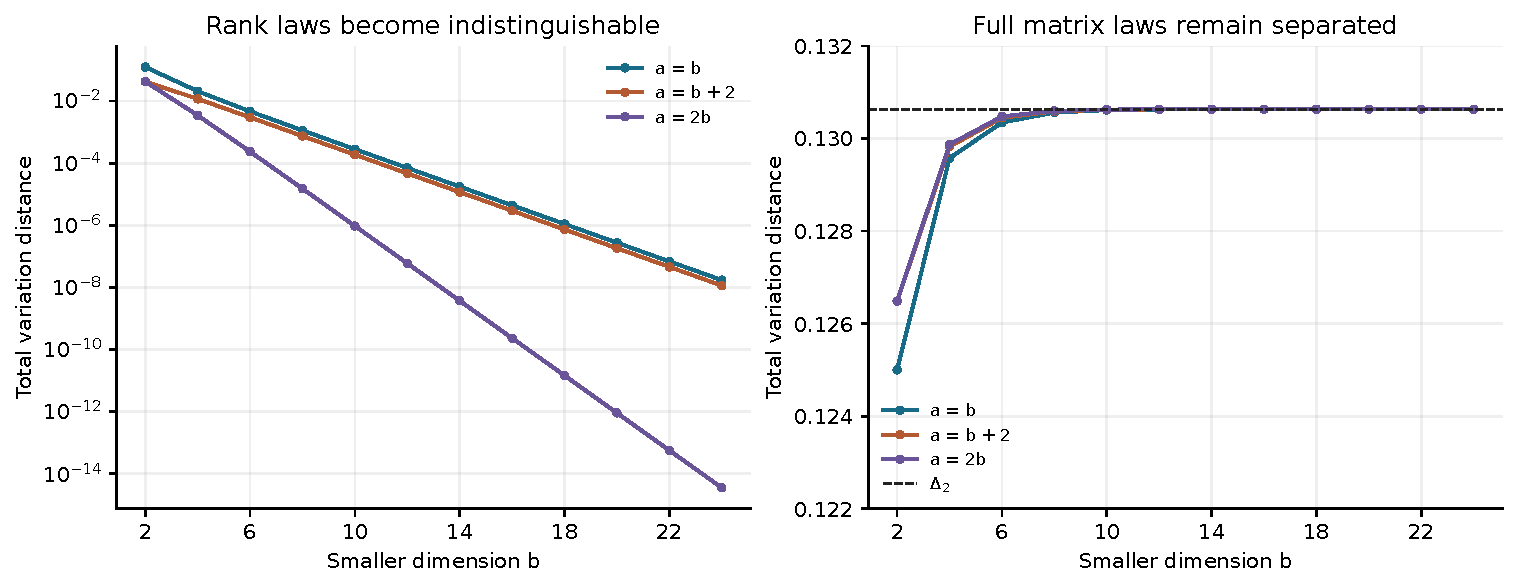
\includegraphics[width=\textwidth]{figures/distances.pdf}
\caption{Exact finite laws over $\F_2$ for three dimension schedules.
The rank-distance axis is logarithmic. The full distance converges to the
same positive constant at every displayed aspect ratio.}
\label{fig:distances}
\end{figure}

\subsection{Commands and contents}

From the archive directory, the commands are
\begin{verbatim}
python3 code/verify.py
python3 code/exhaustive_check.py
python3 code/make_figure.py
pdflatex paper.tex
pdflatex paper.tex
\end{verbatim}
The first two scripts need only Python's standard library. The figure script
needs matplotlib. The PDF build uses ordinary LaTeX packages listed in the
preamble; the figure is included in the archive, so rebuilding the paper
does not require matplotlib. The archive also contains the inspected source
snapshots, commit and blob metadata, a source audit, a formalization roadmap,
and SHA-256 checksums.

\section{Verification status and remaining scope}

The manuscript gives a complete human-readable proof. Its moment formulas,
leading coefficients, and dimension-uniform error estimates were derived
and checked independently during preparation. Exact rational computation
and exhaustive enumeration test the finite formulas. Neither method
replaces the general proof, and no new Lean kernel check is claimed.
\texttt{FORMALIZATION.md} identifies the finite algebra, moment inversion,
and summability lemmas that a Lean formalization would need.

The inspected source concerns RH and GRH for \emph{Dirichlet} $L$-functions.
The pinned upstream revision is
\texttt{72fead102f663d5c7a407964a13dc0cf9d977207}.
The live verification report by Andrew Sutherland \cite{Sutherland},
updated on 27 November 2026, records successful builds, kernel replays,
statement comparisons, and external-checker acceptance for that revision.
Those checks were read, not rerun here. The new theorem proved in this note
has no dependency on a zero theorem and is valid by finite algebra and
the estimates given above.

The result settles the complementary \emph{nondegenerate} rectangular
portion of \texttt{spn:q:symplectic}. The broader source question, in which
radicals and an independent complement dimension grow simultaneously,
remains outside the theorem. The exact optimal rank-only event at every
finite dimension is also not asserted: full column rank is proved
asymptotically optimal. The residual singularity event for the full matrix,
in contrast, is exactly optimal by Proposition~\ref{prop:likelihood}.

\begin{thebibliography}{9}
\raggedright
\bibitem{ProveIt}
Vladimir Reshetnikov, \emph{ProveIt: Beyond the Riemann hypothesis for
Dirichlet $L$-functions: consequences, transfers and limits}.
Inspected revision \texttt{497c1844e71393df41914f5b783d5dc9a618eb61},
27 November 2026. See the symplectic section and its labels listed in
Section~1.\newline
\url{https://github.com/VladimirReshetnikov/ProveIt/tree/497c1844e71393df41914f5b783d5dc9a618eb61/Analysis/GeneralizedRiemannHypothesis/Article}

\bibitem{FulmanGoldstein}
Jason Fulman and Larry Goldstein, \emph{Stein's method and the rank
distribution of random matrices over finite fields}, Annals of Probability
\textbf{43} (2015), 1274--1314.\newline
\url{https://doi.org/10.1214/13-AOP889};
\url{https://arxiv.org/abs/1211.0504}.

\bibitem{DeBoeck}
Maarten De Boeck and Geertrui Van de Voorde,
\emph{Anzahl theorems for trivially intersecting subspaces generating a
non-singular subspace I: symplectic and hermitian forms},
Linear Algebra and its Applications \textbf{699} (2024), 367--402.\newline
\url{https://doi.org/10.1016/j.laa.2024.07.004};
\url{https://arxiv.org/abs/2407.07486}.

\bibitem{Sutherland}
Andrew Sutherland, \emph{Verification files for the shorter Lean proof of RH
and of GRH for Dirichlet $L$-functions}. Updated 27 November 2026,
17:27 UTC; accessed 27 November 2026.\newline
\url{https://math.mit.edu/~drew/shortgrh/}.
\end{thebibliography}
\end{document}
